
  \subsection*{Rappel théorique}
  
  Dans le cadre de ce TP, nous allons faire une analyse externe de l'environnement de Decathlon. Nous allons nous appuyer sur les analyses PESTEL et des 5 forces de Porter.
  
    \begin{figure}[H]
      \centering
        \definecolor{ccqqqq}{rgb}{0.8,0,0}
        \definecolor{zzttqq}{rgb}{0.6,0.2,0}
        \definecolor{ffffww}{rgb}{1,1,0.4}
        \begin{tikzpicture}[line cap=round,line join=round,>=triangle
            45,x=1.0cm,y=1.0cm]
            \clip(1,1) rectangle (12,12);
            \fill[color=ffffww,fill=ffffww,fill opacity=0.5] (1,12) --
            (12,12) -- (12,1) -- (1,1) -- cycle;
            \fill[color=zzttqq,fill=zzttqq,fill opacity=0.35] (2,10) --
            (2,2) -- (11,2) -- (11,10) -- cycle;
            \fill[color=zzttqq,fill=zzttqq,fill opacity=0.3] (3,8) --
            (10,8) -- (10,3) -- (3,3) -- cycle;
            \fill[color=ccqqqq,fill=ccqqqq,fill opacity=0.5] (4,6) --
            (4,5) -- (9,5) -- (9,6) -- cycle;
            \draw [color=ffffww] (1,12)-- (12,12);
            \draw [color=ffffww] (12,12)-- (12,1);
            \draw [color=ffffww] (12,1)-- (1,1);
            \draw [color=ffffww] (1,1)-- (1,12);
            \draw [color=zzttqq] (2,10)-- (2,2);
            \draw [color=zzttqq] (2,2)-- (11,2);
            \draw [color=zzttqq] (11,2)-- (11,10);
            \draw [color=zzttqq] (11,10)-- (2,10);
            \draw [color=zzttqq] (3,8)-- (10,8);
            \draw [color=zzttqq] (10,8)-- (10,3);
            \draw [color=zzttqq] (10,3)-- (3,3);
            \draw [color=zzttqq] (3,3)-- (3,8);
            \draw (4.16,11.36) node[anchor=north west]
            {Macro-environnement};
            \draw (5.27,9.3) node[anchor=north west] {Industrie};
            \draw (5.24,7.24) node[anchor=north west] {Concurrents};
            \draw (5.1,5.79) node[anchor=north west] {L'organisation};
            \draw (5.54,4.55) node[anchor=north west] {Marchés};
            \draw [color=ccqqqq] (4,6)-- (4,5);
            \draw [color=ccqqqq] (4,5)-- (9,5);
            \draw [color=ccqqqq] (9,5)-- (9,6);
            \draw [color=ccqqqq] (9,6)-- (4,6);
        \end{tikzpicture}
      \caption{Les couches de l'environnement externe d'une entreprise}
    \end{figure}
    
    \bigskip
    
    \begin{figure}[H]
      \begin{center}
	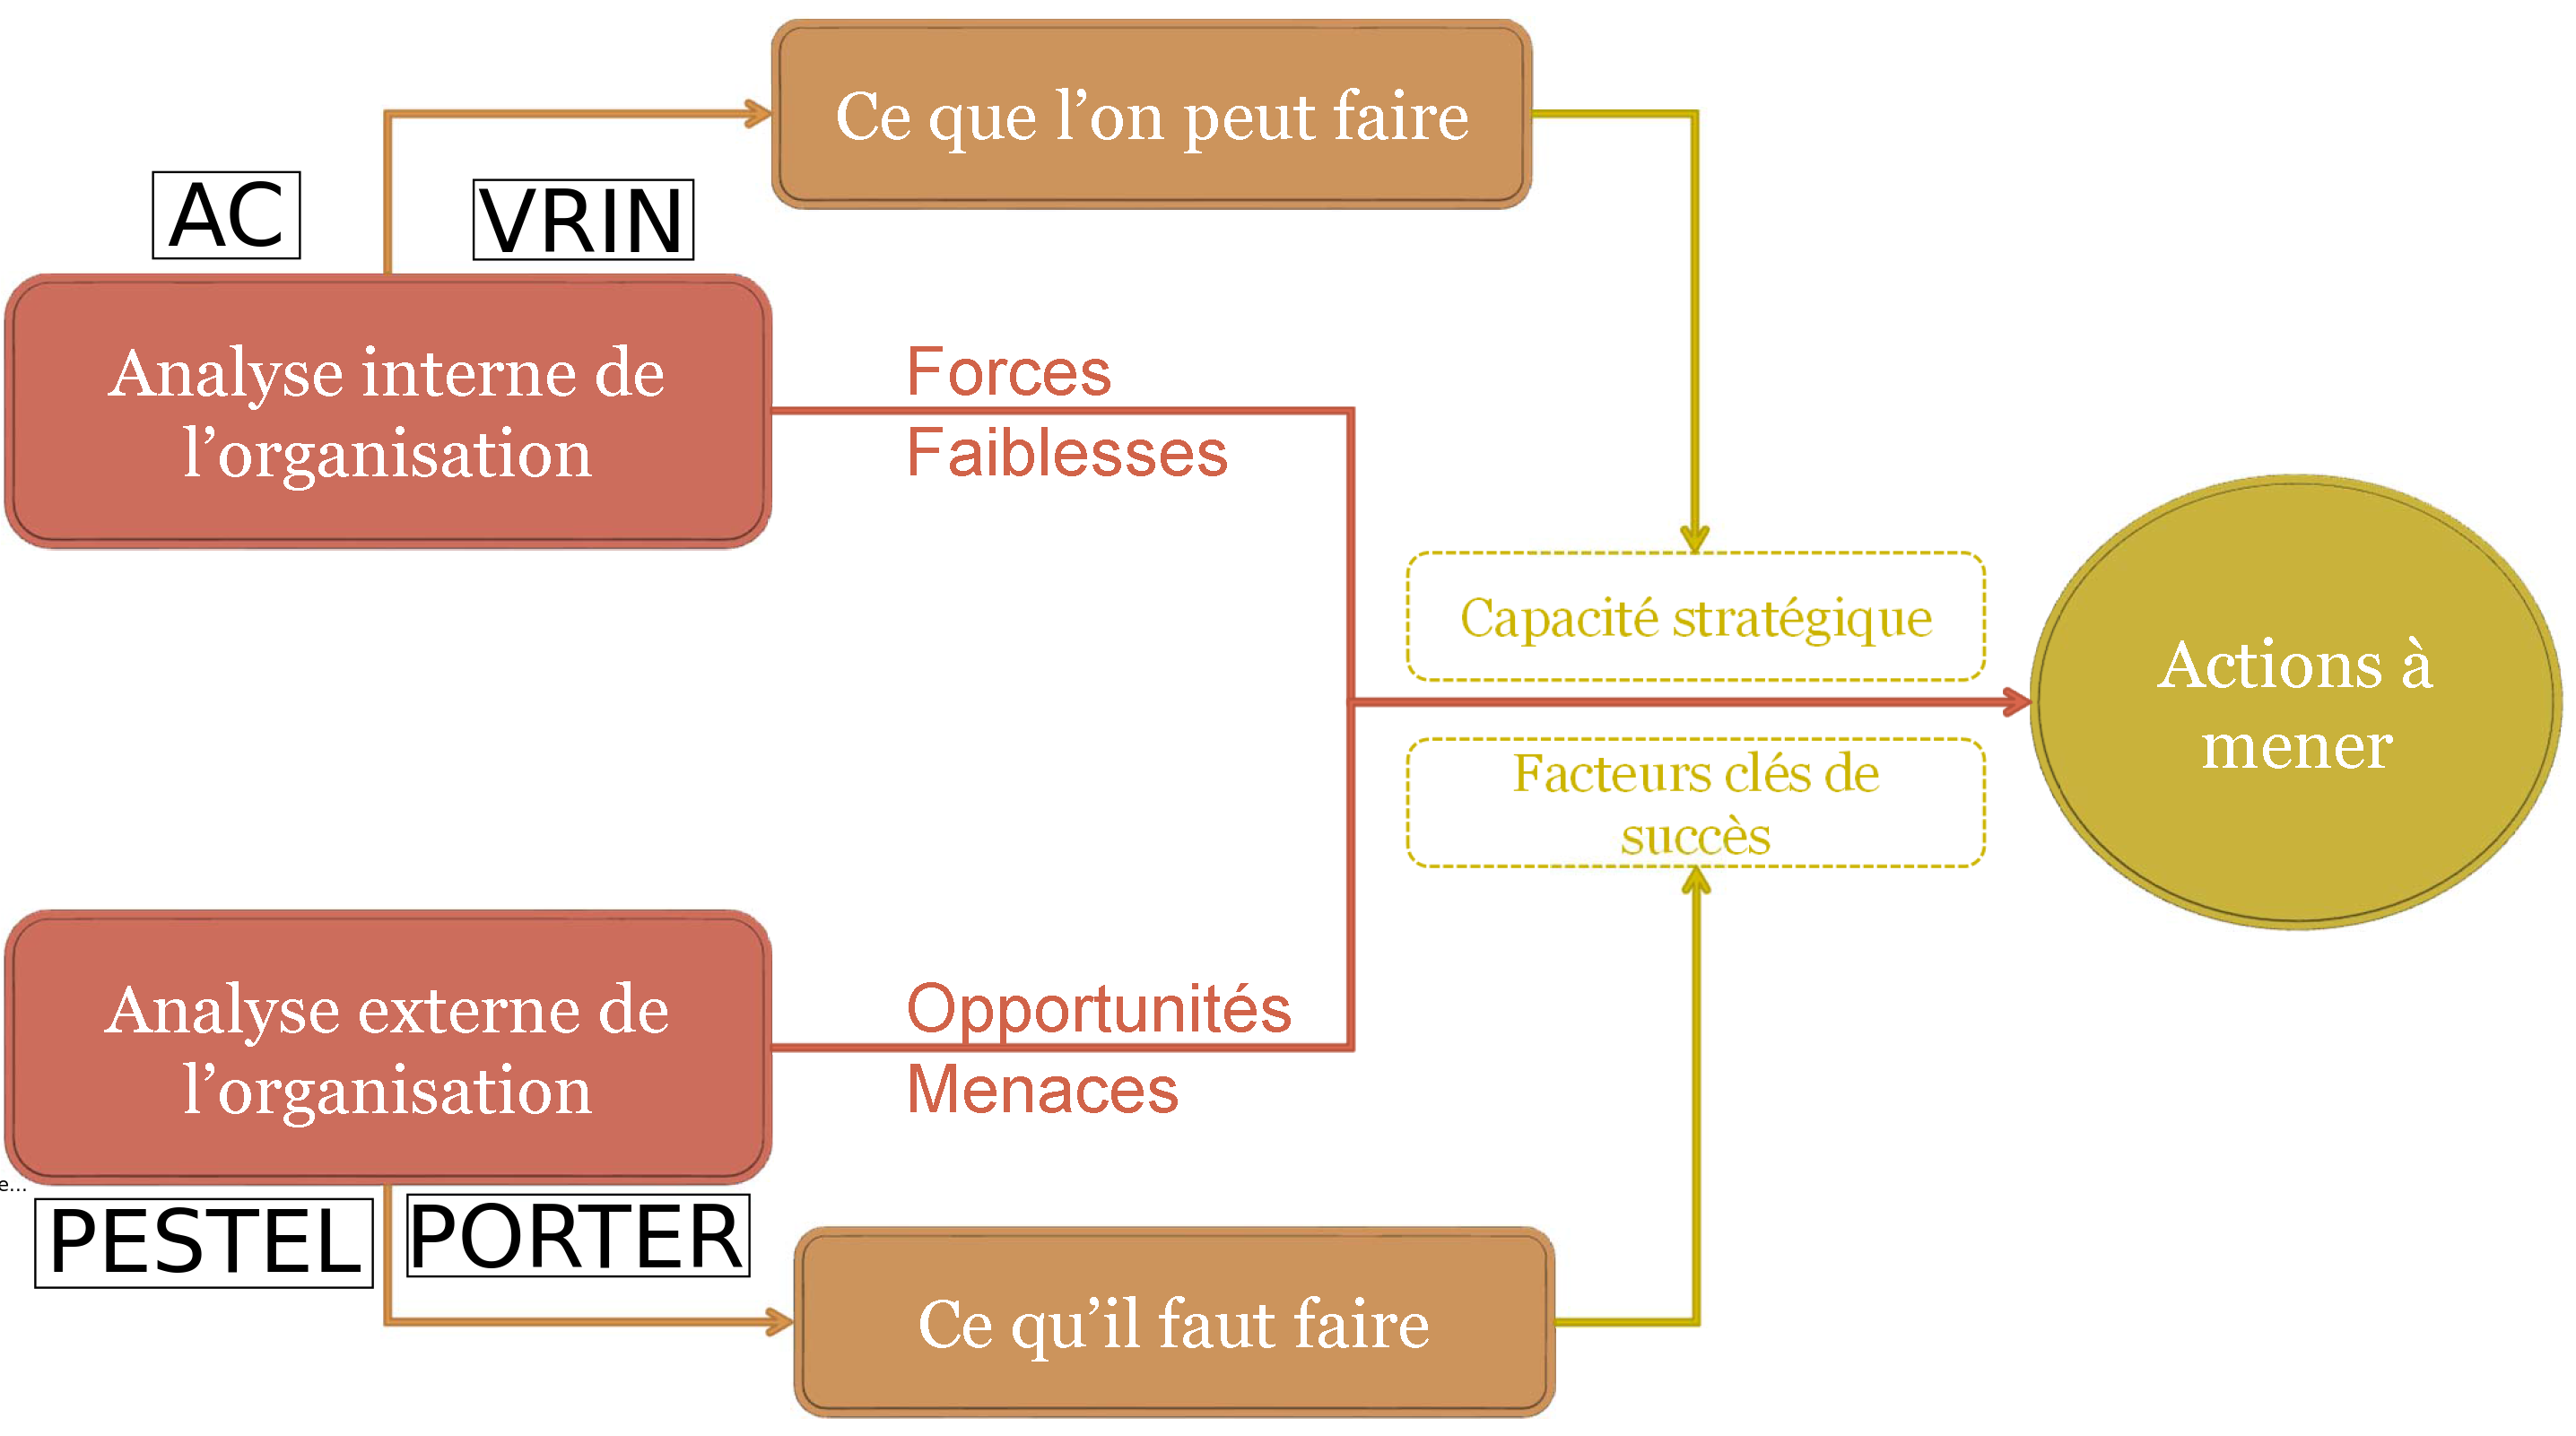
\includegraphics[width=\linewidth]{analyse_swot.png}
	\caption{Mécanisme de l'analyse SWOT}
      \end{center}
    \end{figure}
    
    \bigskip
    
    \subsubsection{L'analyse PESTEL}
    
    L'analyse PESTEL comprend 3 étapes :
    
    \begin{enumerate}
     \item Identifier les facteurs économiques
     \item Dégager les tendances lourdes (variables pivots)
     \item Elaboration de scénarios
    \end{enumerate}
    
    \begin{center}
         \framebox{\begin{minipage}{0.18\linewidth} 
	  \begin{description}
	  \item[P]olitique
	  \item[E]conomique
	  \item[S]ocial
	  \item[T]echnologique
	  \item[E]cologique
	  \item[L]égal
	  \end{description}
	 \end{minipage}}
    \end{center} \bigskip
    
    \begin{table}[!ht]
      \begin{center}
	\begin{tabular}{|>{\centering\arraybackslash}P{5cm}||>{\centering\arraybackslash}P{5cm}||>{\centering\arraybackslash}P{5cm}|}
	 \hline
	   \textbf{P} &  \textbf{E} & \textbf{S} \\ \hline
	  \begin{itemize} 
	  \item Primes 
	  \item Réductions fiscales 
	  \item Directives européennes contre les émissions de $CO_{2}$
	  \end{itemize}
	  & 
	  \begin{itemize} 
	  \item Coûts de l'énergie
	  \item Taux de croissance de l'économie
	  \item Investissements dans l'immobilier
	  \end{itemize}
	  & 
	  \begin{itemize}
	  \item Achats produits verts
	  \item Mode de vie à consommation zéro
	  \end{itemize} \\  \hline
	   \textbf{T} &  \textbf{E} & \textbf{L} \\ \hline
	  \begin{itemize}
	   \item R\&D avancée sur les panneaux solaires (design, performance)
	  \end{itemize}
	  &
	  \begin{itemize}
	   \item Disparition des ressources fossiles
	   \item Importance accordée aux énergies renouvelables
	  \end{itemize}
	  &
	  \begin{itemize}
	   \item Droit de polluer
	   \item Certificats verts
	   \item Permis d'urbanisme
	  \end{itemize} \\ \hline
	  
	\end{tabular}
	
	\caption{Illustration de PESTEL sur l'industrie des toitures solaires}
      \end{center}
    \end{table}
    
    \begin{figure}[H]
      \begin{center}
	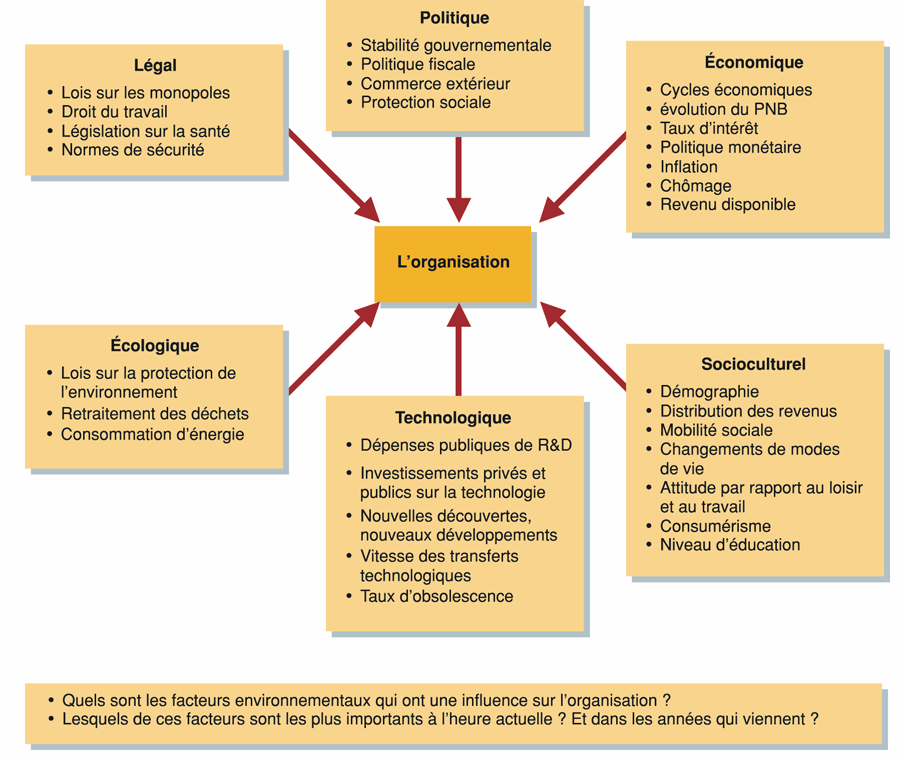
\includegraphics[width=\linewidth]{analyse_pestel.png}
	\caption{Principaux thèmes ressortant d'une analyse PESTEL}
      \end{center}
    \end{figure}
   
    \begin{figure}[H]
        \centering
        \definecolor{ffffff}{rgb}{1,1,1}
        \definecolor{dawvuc}{rgb}{0.85,0.4,0.3}
        \definecolor{csdqdw}{rgb}{0.76,0.82,0.84}
        \begin{tikzpicture}[line cap=round,line join=round,>=triangle
            45,x=1.0cm,y=1.0cm]
            \clip(0.2,0.5) rectangle (10,10);
            \fill[color=dawvuc,fill=dawvuc,fill opacity=1.0] (7,9.5) --
            (7,6.5) -- (9.5,6.5) -- (9.5,9.5) -- cycle;
            \fill[color=csdqdw,fill=csdqdw,fill opacity=1.0] (2.75,9.54)
            -- (2.75,6.54) -- (5.25,6.54) -- (5.25,9.54) -- cycle;
            \fill[color=csdqdw,fill=csdqdw,fill opacity=1.0] (2.75,5.51)
            -- (2.75,2.51) -- (5.25,2.51) -- (5.25,5.51) -- cycle;
            \fill[color=csdqdw,fill=csdqdw,fill opacity=1.0] (6.99,5.51)
            -- (6.99,2.51) -- (9.49,2.51) -- (9.49,5.51) -- cycle;
            \draw [->,line width=5.2pt] (2,2) -- (10,2);
            \draw [->,line width=5.2pt] (2,2) -- (2,10);
            \draw [->,line width=2.8pt,color=csdqdw] (2,6) -- (10,6);
            \draw [->,line width=2.8pt,color=csdqdw] (6,2) -- (6,10);
            \draw [color=dawvuc] (7,9.5)-- (7,6.5);
            \draw [color=dawvuc] (7,6.5)-- (9.5,6.5);
            \draw [color=dawvuc] (9.5,6.5)-- (9.5,9.5);
            \draw [color=dawvuc] (9.5,9.5)-- (7,9.5);
            \draw [color=ffffff](7.4,8.7) node[anchor=north west]
            {\parbox{1.57 cm}{\centering \Large Key Drivers}};
            \draw [color=csdqdw] (2.75,9.54)-- (2.75,6.54);
            \draw [color=csdqdw] (2.75,6.54)-- (5.25,6.54);
            \draw [color=csdqdw] (5.25,6.54)-- (5.25,9.54);
            \draw [color=csdqdw] (5.25,9.54)-- (2.75,9.54);
            \draw [color=csdqdw] (2.75,5.51)-- (2.75,2.51);
            \draw [color=csdqdw] (2.75,2.51)-- (5.25,2.51);
            \draw [color=csdqdw] (5.25,2.51)-- (5.25,5.51);
            \draw [color=csdqdw] (5.25,5.51)-- (2.75,5.51);
            \draw [color=csdqdw] (6.99,5.51)-- (6.99,2.51);
            \draw [color=csdqdw] (6.99,2.51)-- (9.49,2.51);
            \draw [color=csdqdw] (9.49,2.51)-- (9.49,5.51);
            \draw [color=csdqdw] (9.49,5.51)-- (6.99,5.51);
            \draw (0.7,8) node[anchor=north west] {Elevé};
            \draw (7,1.75) node[anchor=north west] {Elevée};
            \draw (3,1.75) node[anchor=north west] {Faible};
            \draw (0.7,4) node[anchor=north west] {Faible};
            \draw (0,6.12) node[anchor=north west] {\Large
                \textbf{Impact}};
            \draw (4.8,1.3) node[anchor=north west] {\Large
                \textbf{Incertitude}};
        \end{tikzpicture}
    \end{figure}

   \begin{multicols}{2}
    
    \enquote{Les \textbf{key drivers} (ou \textit{variables pivots})
    sont des facteurs de l'environnement qui sont enclins à avoir un
grand impact sur la réussite ou l'échec d'une stratégie.}
    \bigskip
    
    Un scénario est une représentation plausible de différents futurs envisageables, obtenue à partir de la combinaison des key drivers (de variables pivots incertaines).
    
   \end{multicols}
   
   \subsubsection{L'analyse de Porter}
   
   La filière industrielle est l'ensemble des liens inter-organisationnels et des activités nécessaires à la création d'un produit/service. Dans cette filière, nous différencierons les acteurs selon leur place par rapport à l'entreprise étudiée. Les fournisseurs sont en \textit{amont} de la chaîne et les clients sont en \textit{aval} par rapport à l'entreprise.
   
   \begin{figure}[H]
      \begin{center}
	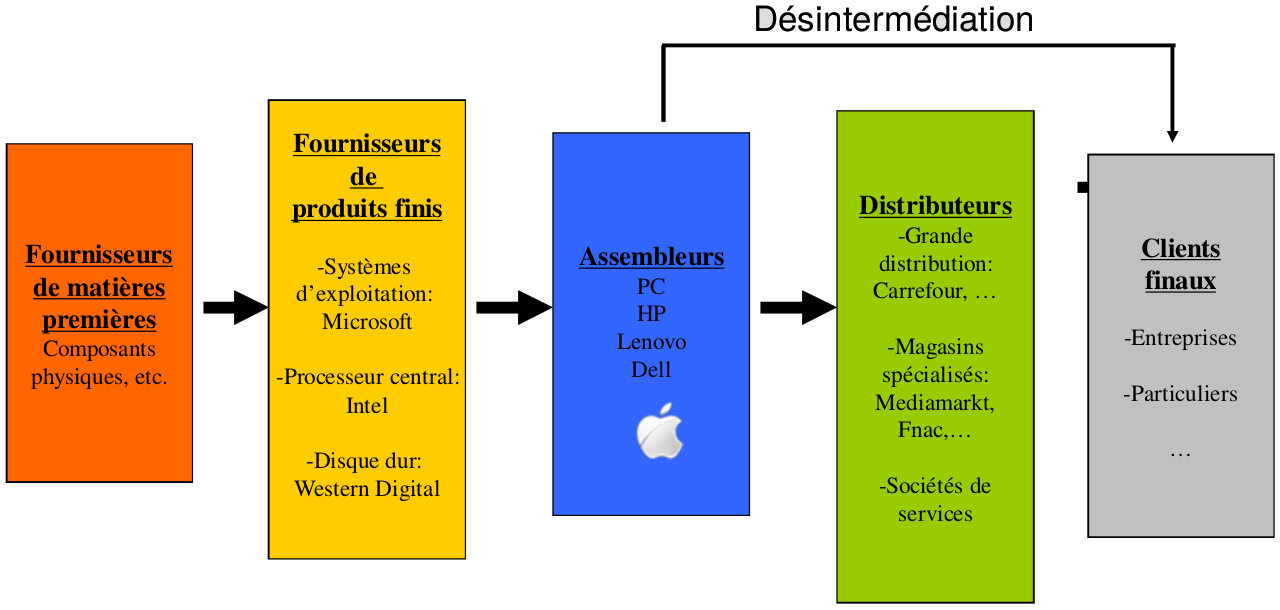
\includegraphics[width=\linewidth]{filiere_industrielle_ordinateur.png}
	\caption{Exemple de filière industrielle pour les ordinateurs}
      \end{center}
   \end{figure}
   
   Dans la filière industrielle pour les ordinateurs, on se rend compte
   que les assembleurs deviennent également distributeurs (intégration
   vers l'aval du point de vue des assembleurs) par la vente sur
   internet et la création de magasin de la marque (Apple Store). Ce
   phénomène est appelé la \enquote{désintermédiation}.
   
   \begin{figure}[H]
      \begin{center}
	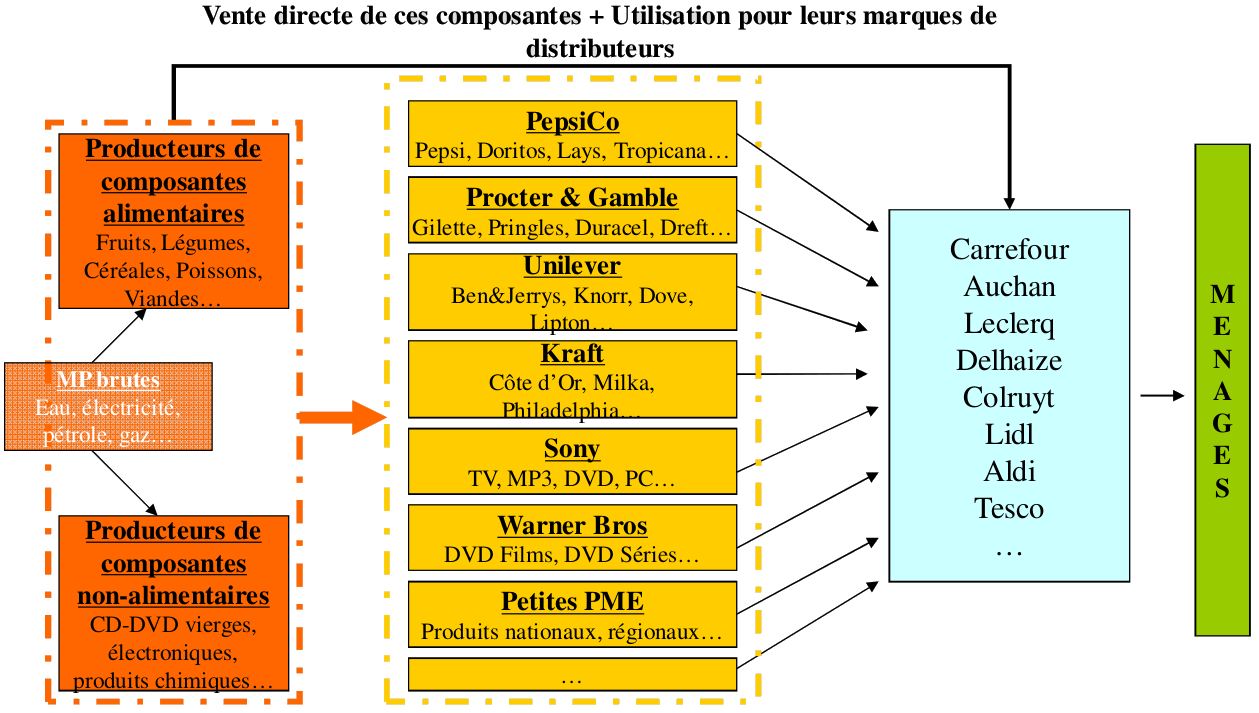
\includegraphics[width=\linewidth]{filiere_industrielle_grande_distribution.png}
	\caption{Exemple de la filière industrielle pour la grande distribution}
      \end{center}
   \end{figure}
   
   Le modèle des 5 forces a pour objectif de fournir une description de la structure de l'industrie afin d'envisager le potentiel profit dans cette industrie.
   
   \underline{{\textbf{ou}}}
   
   Le modèle des 5 forces de Porter permet d'évaluer l'attractivité d'une industrie en termes d'intensité concurrentielle.
   
   Une \textit{industrie} est un groupe d'organisations proposant la même offre de biens ou de services.
   
   \begin{figure}[H]
      \begin{center}
	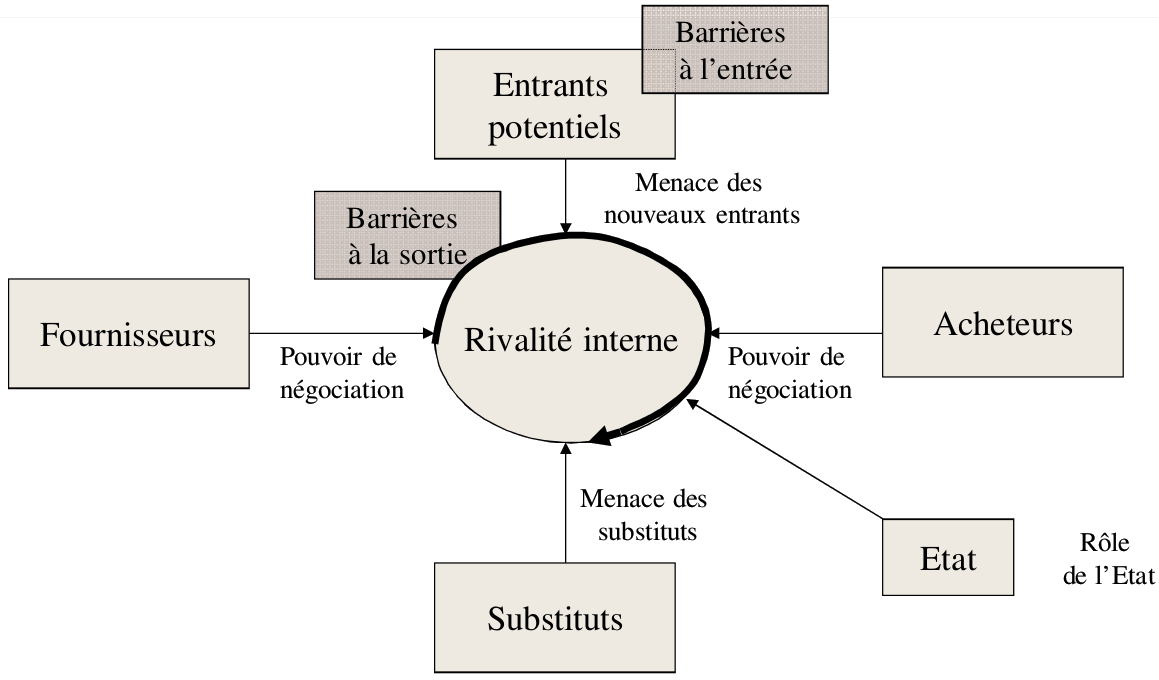
\includegraphics[width=\linewidth]{modele_de_porter.png}
	\caption{Représentation des 5+1 forces du modèle de Porter}
      \end{center}
   \end{figure}
   
   Les 5 forces sont :
   
   \begin{enumerate}
    \item Les entrants potentiels
    \item Les clients
    \item Les substituts
    \item Les fournisseurs
    \item Les concurrents directs
   \end{enumerate}
   
   Nous rajoutons à ce modèle trop américain la présence de l'Etat.
   
   \begin{figure}[H]
      \begin{center}
	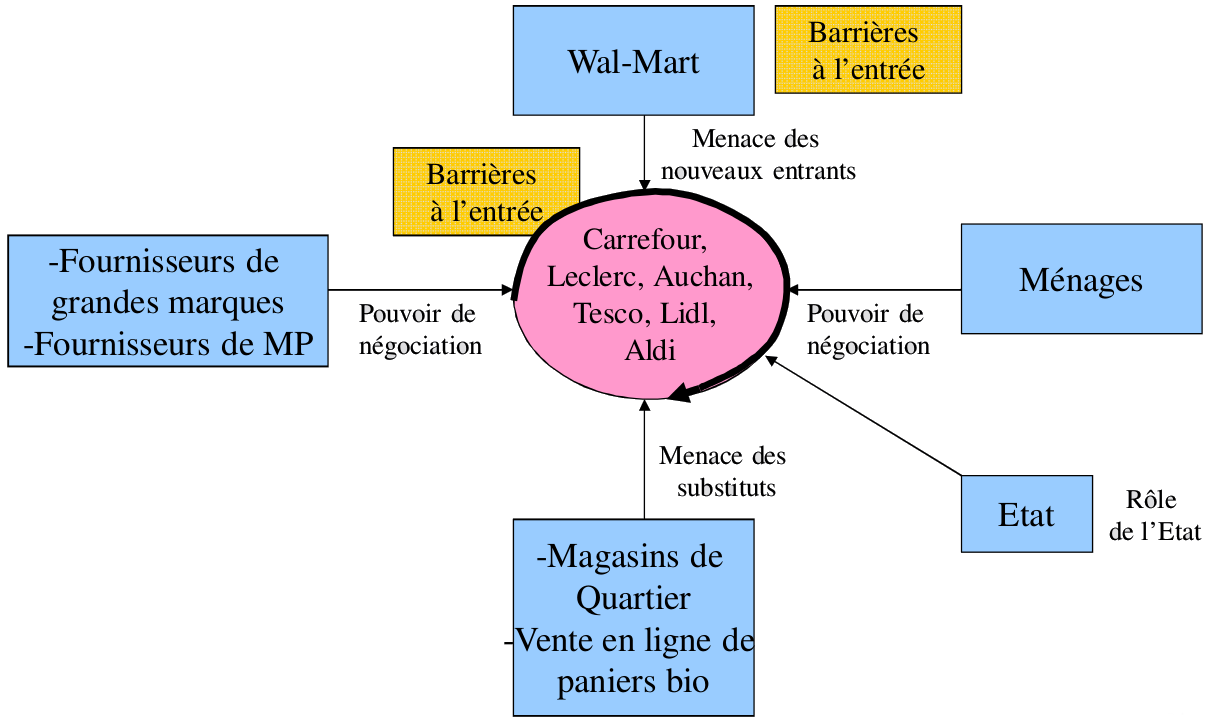
\includegraphics[width=\linewidth]{5_forces_grande_distribution.png}
	\caption{Le modèle des 5 forces appliqué à la grande distribution}
      \end{center}
   \end{figure}
   
   Parmi les limites du modèle de Porter, les principales sont :
   
   \begin{itemize}
    \item Pas de prise en compte des partenariats et des alliances entre organisations
    \item Approche statique (photographie à un moment précis)
    \item Le niveau d'analyse
   \end{itemize}
   
   \subsubsection{Les facteurs clés de succès}
      L'identification des FCS est la conclusion logique d'une analyse des 5+1 forces de Porter
      
      \enquote{Les facteurs clés de succès sont les éléments stratégiques qu'une organisation doit maîtriser afin d'assurer sa pérénnité dans le secteur.}
  
  \clearpage
  
  \subsection{Application pratique : Decathlon}
  
  Decathlon est un groupe de distribution d'articles de sport du groupe Oxylane. Decathlon dispose de nombreuses marques comme Quechua, Nabaji, Tribord, wed'ze, Domyos,...
  
    \subsubsection{Historique}
      \begin{description}
	\item[1976] Michel \textsc{Leclercq} fonde Decathlon
	  \subitem Le premier magasin ouvre ses portes à Englos dans le Nord de la France avec un concept clair : regrouper sous un même toit tous les sports, au meilleur prix et en libre service.
	\item[1985] Création de l'Université Internationale des métiers
	  \subitem Lancement de l'Actionariat pour tous les salariés
	\item[1986] Création de \enquote{Décathlon Production}
	\item[1992] Ouverture à Barcelone
	\item[1993] Ouverture à Milan
	  \subitem 5000 collaborateurs / 100 magasins
	\item[1996] Création des premières Marques Passion (Quechua/Tribord)
	  \subitem 10000 collaborateurs
	\item[1997] Ouverture à Anvers
	\item[2000] Ouverture à Londres, Amsterdam, Lisbonne
	\item[2001] Ouverture à Varsovie, Sao Paulo
	  \subitem 25000 collaborateurs / 300 magasins
	\item[2003] Ouverture du premier magasin en Chine, à Shangaï
	  \subitem Décathlon crée les \enquote{évènements clients acteurs}
	\item[2006] Ouverture à Moscou
	\item[2008] Décathlon devient une enseigne du réseau Oxylane
	\item[2010] Ouverture de la Turquie et de la République Tchèque
	  \subitem 50000 collaborateurs / 535 magasins
      \end{description}

    \subsubsection{La vision}
	Créer l'envie et rendre accessibles au plus grand nombre le plaisir et les bienfaits du sport.
	
    \subsubsection{Quelques chiffres}
      
      \begin{tabular}{lll}
	  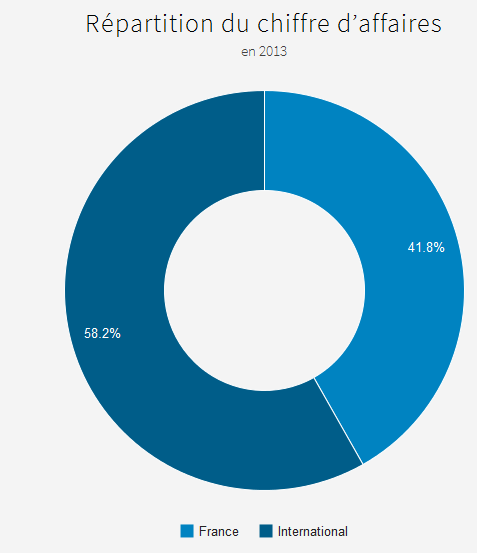
\includegraphics[width=0.3\linewidth]{repartition_CA_decathlon.png}
	&
	  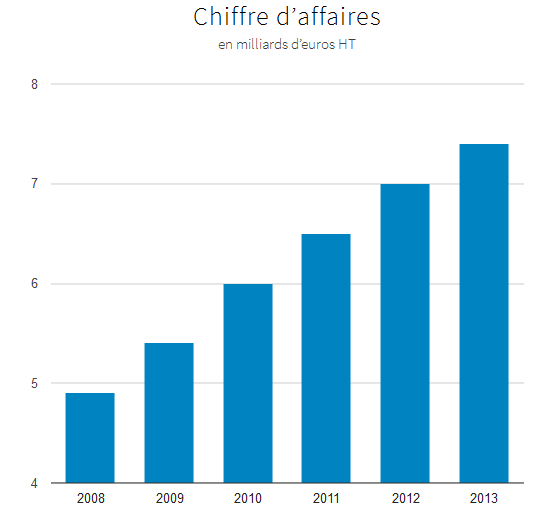
\includegraphics[width=0.3\linewidth]{CA_decathlon.png}
	&
	  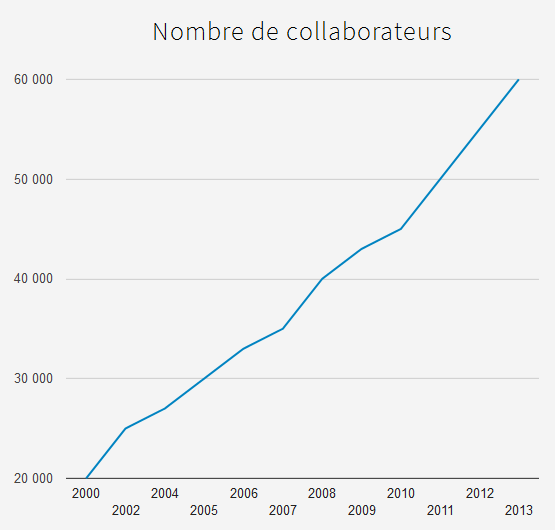
\includegraphics[width=0.3\linewidth]{collaborateurs_decathlon.png}
	\\
      \end{tabular}
      
    \subsubsection{Analyse PESTEL}
    
        \begin{table}[!ht]
      \begin{center}
	\begin{tabular}{|>{\centering\arraybackslash}P{5cm}||>{\centering\arraybackslash}P{5cm}||>{\centering\arraybackslash}P{5cm}|}
	 \hline
	   \textbf{P}olitique &  \textbf{E}conomique & \textbf{S}ociologique \\ \hline
	  \begin{itemize} 
	  \item Quotas à l'importation 
	  \item Lobbying des associations pour la défense des ouvriers
	  \end{itemize}
	  & 
	  \begin{itemize} 
	  \item Réduction du temps de travail (35h) permettant de pouvoir faire du sport
	  \item Pouvoir d'achat (360\euro{}/an)
	  \item Hard discount (montée en puissance des marques blanches)
	  \end{itemize}
	  & 
	  \begin{itemize}
	  \item Effet sportswear
	  \item Evolution d'une pratique moins encadrée, en famille ou entre amis
	  \item Importance croissante accordée à l'image de soi
	  \item Démographie (le développement urbain pousse à la construction de centre sportif)
	  \end{itemize} \\  \hline
	   \textbf{T}echnologique &  \textbf{E}cologique & \textbf{L}égal \\ \hline
	  \begin{itemize}
	   \item Evolution des technologies
	   \item Vente en ligne (développement e-commerce)
	  \end{itemize}
	  &
	  \begin{itemize}
	   \item Recherche d'une proximité croissante avec la nature
	   \item Conditions climatiques
	   \item Impact environnemental (production et transport $CO_{2}$
	  \end{itemize}
	  &
	  \begin{itemize}
	   \item Droit de la concurrence
	   \item Législation relative aux implantations de nouveaux magasins
	   \item Normes de sécurité
	  \end{itemize} \\ \hline
	  
	\end{tabular}
	
	\caption{Illustration de PESTEL sur l'industrie de la distribution d'article de sport}
      \end{center}
    \end{table}
    
    \subsubsection{Key drivers et scenarios}
    
    \begin{figure}[H]
      \centering
	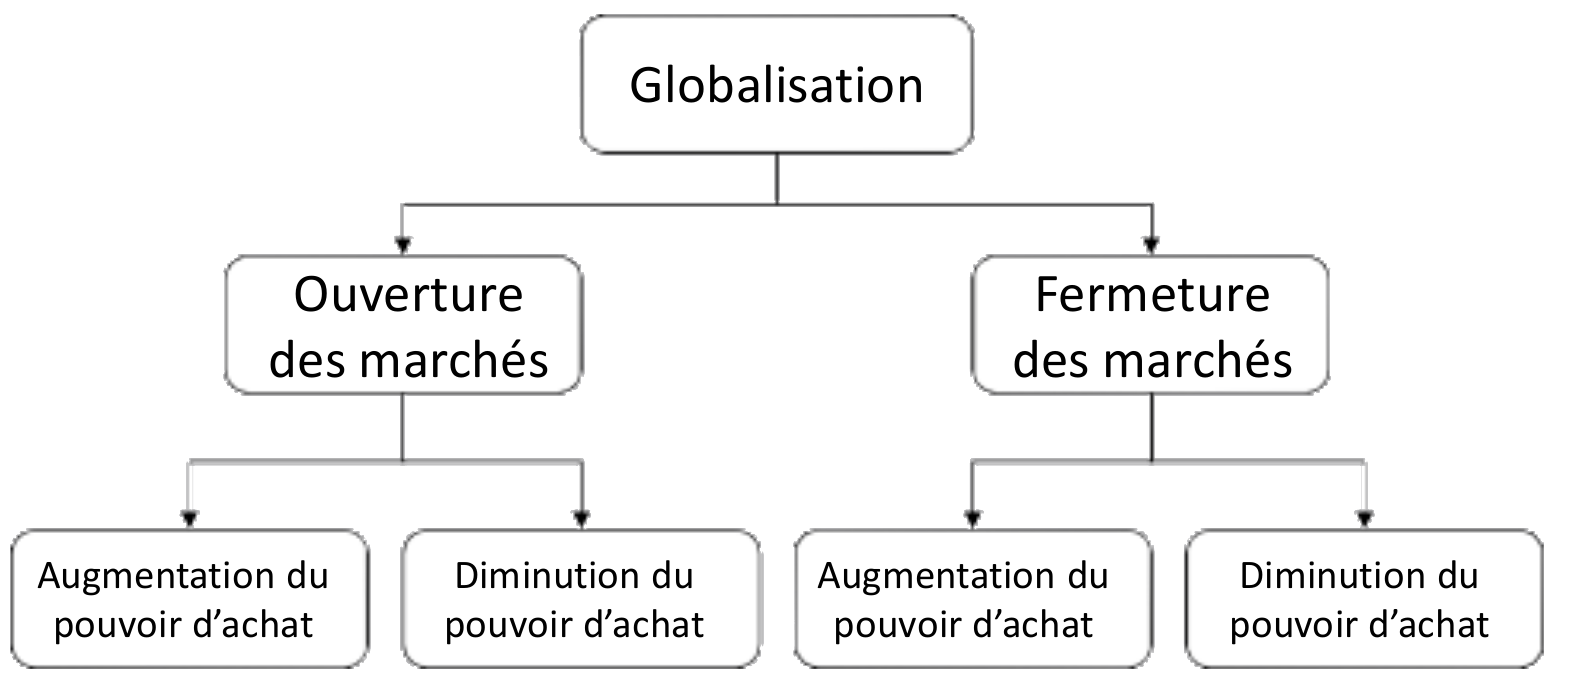
\includegraphics[width=0.5\linewidth]{key_drivers_decathlon.png}
	\caption{Key drivers et scénarios de l'industrie de distribution d'articles de sport}
    \end{figure}
    
    \paragraph{Recommandations} Les recommandants selon les scénarios :
    
    \begin{itemize}
     \item Ouverture des marchés
      \subitem Maximiser la sous-traitance et délocaliser la production
     \item Fermeture des frontières
      \subitem Relocalisation en Europe
      \subitem Maintien des goûts locaux des consommateurs
     \item Diminution du pouvoir d'achat
      \subitem Développement de MDD
      \subitem Réduction de la gamme
      \subitem Maintien des coûts de productions les plus bas
     \item Augmentation du pouvoir d'achat
      \subitem Innovation, recherche et développement
      \subitem Opter pour une stratégie de niche
    \end{itemize}
    
    \subsubsection{Analyse de la filière industrielle}
    
    \begin{figure}[H]
      \begin{center}
	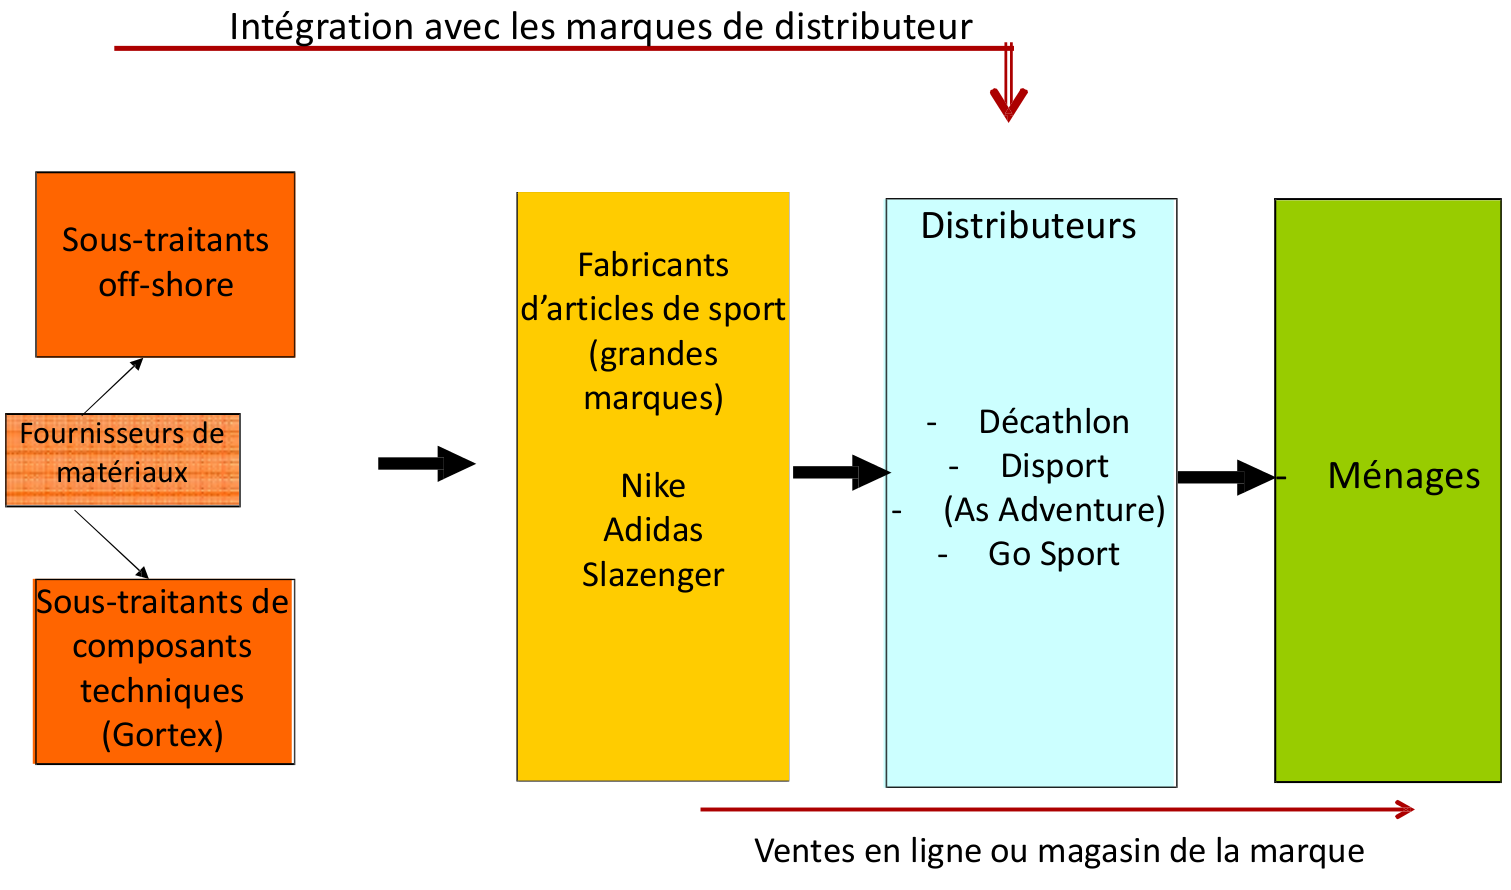
\includegraphics[width=\linewidth]{filiere_industrielle_decathlon.png}
	\caption{Filière industrielle de la distribution d'articles de sport}
      \end{center}
    \end{figure}
    
    \clearpage
    
    \subsubsection{Analyse des 5+1 forces}
    
    \begin{figure}[H]
      \begin{center}
	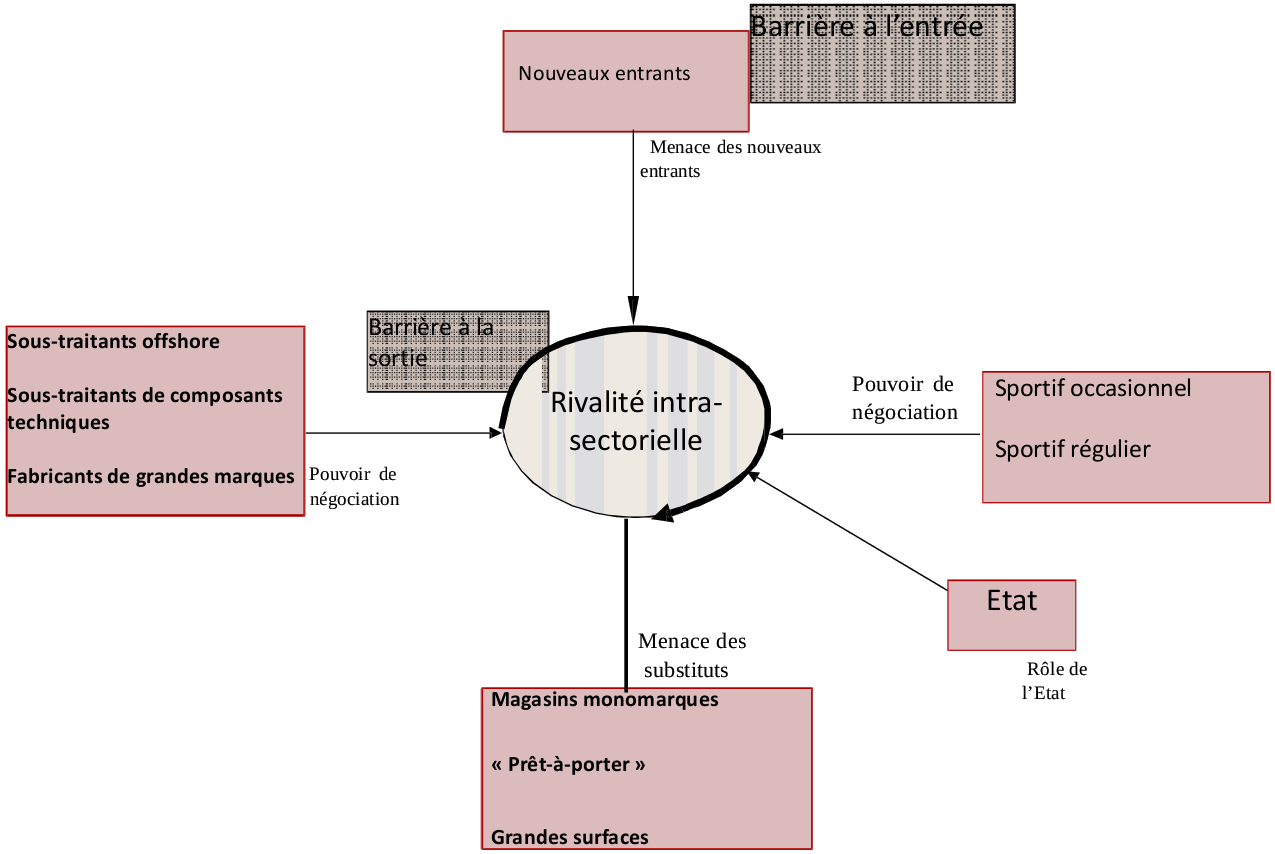
\includegraphics[width=\linewidth]{5_forces_decathlon.png}
	\caption{Analyse des 5+1 forces de Porter pour la distribution d'articles de sport}
      \end{center}
    \end{figure}
    
    \paragraph{Intensité concurrentielle} Il y a de grosses barrières à la sortie.
    
    \begin{table}[!ht]
      \begin{center}
	\begin{tabular}{p{5cm}|p{5cm}|p{5cm}}
	  Type d'influence & Critères mobilisés & Caractérisation de l'influence \\ \hline
	  Rivalité intra-sectorielle  & Taux de croissance faible (marché à maturité) & \\
	  & Concentration assez forte & \\
	  & Parts de marché et coûts sont clés & \\
	\end{tabular}
	\caption{Analyse de l'intensité concurrentielle}
      \end{center}
    \end{table}
    
    \clearpage

    \paragraph{Menace des nouveaux entrants}
    
    \begin{itemize}
     \item Economie d'échelle
     \item Effet d'expérience
     \item Emplacements stratégiques
     \item Intensité capitalistique (l'investissement nécessaire)
    \end{itemize}
    
    \begin{table}[!ht]
      \begin{center}
	\begin{tabular}{p{3.5cm}|p{5cm}|p{5.5cm}}
	Type d'influence & Critères mobilisés & Caractérisation de l'influence \\ \hline
	  Nouveaux entrants & Fortes barrières à l'entrée & Faible menace \\
	  & Intensité capitalistique & \\
	  & Notoriété & \\
	  & Effet d'expérience & \\
	\end{tabular}
	\caption{Analyse de la menace des nouveaux entrants}
      \end{center}
    \end{table}
    
    \paragraph{Menace des substituts}
    
    \begin{table}[!ht]
      \begin{center}
	\begin{tabular}{p{4cm}|p{5cm}|p{6cm}}
	  Type d'influence & Critères mobilisés & Caractérisation de l'influence \\ \hline
	  Magasins monomarques & Forte substituabilité (marques) & Menace croissante \\
	  & Service, conseil & \\ \hline
	  Prêt-à-porter & Utilisation urbaine des équipements de sport & Menace croissante : textile sportswear \\ \hline
	  Grandes surfaces & Gamme peu profonde et peu technique & Menace faible \\
	\end{tabular}
	\caption{Analyse de la menace des substituts}
      \end{center}
    \end{table} 
    
    \paragraph{Pouvoir de négociation des acheteurs}
    
    \begin{table}[!ht]
      \begin{center}
	\begin{tabular}{p{4cm}|p{6cm}|p{5cm}}
	  Type d'influence & Critères mobilisés & Caractérisation de l'influence \\ \hline
	  Sportif occasionnel & Clients nombreux et peu concentrés & Pouvoir modéré \\
	  & Faible coût de transfert (zappeur) & \\
	  & Diverses sources d'approvisionnement & \\ \hline
	  Sportif régulier & Demande de produits de qualité (marque) & Pouvoir élevé \\
	  & Conseils, services & \\
	\end{tabular}
	\caption{Analyse du pouvoir de négociation des acheteurs}
      \end{center}
    \end{table}
    
    \paragraph{Pouvoir de négociation des fournisseurs}
    
    \begin{table}[!ht]
      \begin{center}
	\begin{tabular}{p{4cm}|p{6cm}|p{5cm}}
	  Type d'influence & Critères mobilisés & Caractérisation de l'influence \\ \hline
	  Sous-traitants offshore & Produits banalisés & Pouvoir de négociation : faible \\
	  & Faible qualité & \\
	  & Facilité de transfert & \\ \hline
	  Sous-traitants de composants techniques & Forte qualité liée & Fort \\
	  & Faible capacité de transfert & \\ \hline
	  Fabricants de grandes marques & Faible capacité de transfert (image de marque) & Fort \\
	  & Capacité d'intégration en amont pour les distributeurs (MDD) & \\
	  & Intégration en aval : ouverture de leurs propres magasins & \\
	\end{tabular}
	\caption{Analyse du pouvoir de négociation des fournisseurs}
      \end{center}
    \end{table}
    
    \subsubsection{Conclusion de l'analyse de Porter et des FCS}
    
    Les forces qui pèsent sur le secteur de la distribution d'articles de sport sont :
    
    \begin{enumerate}
     \item Le pouvoir des fournisseurs
      \subitem FCS : Développer des relations privilégiées avec les fournisseurs / sa propre marque de distributeur
     \item Les menaces des substituts
      \subitem FCS : Offrir une large gamme de produits / Effort en R\&D
     \item L'intensité de la concurrence sectorielle
      \subitem FCS : Fidéliser la clientièle
    \end{enumerate}
